% Chapter Template
\chapter{A Secure Bootstrapping for Constrained Devices} % Main chapter title

\label{Chapter5} % Change X to a consecutive number; for referencing this chapter elsewhere, use \ref{ChapterX}

\lhead{Chapter 5. \emph{A Secure Bootstrapping for Constrained Devices}} % Change X to a consecutive number; this is for the header on each page - perhaps a shortened title

%----------------------------------------------------------------------------------------
%	SECTION 5
%----------------------------------------------------------------------------------------

High amount of heterogeneous devices interoperating together in Internet of Thing (IoT) associate to many challenges on scalability, effectiveness, constrained resources, and security for both researching and industrial sectors. As one of the biggest challenges, secure bootstrapping for constrained devices are exceptionally paid attention by researchers. The term bootstrapping denotes process of configuring a device to properly participate in normal network operation. Bootstrapping is complete when a device receives all settings such as an identity, secret keys, a list of access control, protocol suits and etc. This includes any thing from physical link-layer information to application-layer information~\cite{secureboot}. 

Securing bootstrapping process is essential at the first line of defence strategy. Indeed, the configuration information received in this stage is so sensitive that it should be secured to maintain security and stability of systems. Traditionally, security bootstrapping approaches mainly adopted device pairing protocols, key generation and distribution protocols, or secure configuration. However, in the context of Internet of Things, devices are usually various types and resource-constrained, establishing a secure channel among devices remarkably costs time and efforts. For example, devices don't always provide advanced user interfaces to input necessary information. The problem additionally enlarges when a controller and other devices do not have any prior knowledge about a new device. Furthermore, the scale of IoT networks might be sufficiently large, human assistance is expensive and low efficient in such networks. Current approaches partly offer solutions for such problems. 

To provide flexibility, secure bootstrapping schemes should concern on both secure physical access and secure network access. Secure physical access describes devices joining the network must physically authenticate to a trusted center at the first place while secure network access describes the devices must authenticate to other authenticated and authorised devices in the network.  
However, problems may come from users when they accidentally add rouge devices into their network, that happens if they bought used or ingenious devices. Therefore, device registration must be regarded. 

According to our review, the existing approaches partly tackled the problems. Hence, this chapter offers a novel solution for secure bootstrapping schemes in Internet of Things that focuses on security, adaptability, constrained resources. Precisely, our goals are providing a secure configuration between a new device and a controller, and a trust relationship among devices, even in some worst cases when controllers are unaccessible, when the devices are reused, and when the introducer could be lost. 

The rest of this chapter is organised as follows. The first section introduces requirements for bootstrapping schemes for constrained devices.  In section~\ref{envi}, we defined environment, problems, attacker model, and notations. Then, section~\ref{buildingblocks} discusses about secure bootstrapping building blocks and related work. In section~\ref{proposal}, we introduce our secure bootstrapping scheme for constrained devices in IoT. Section~\ref{validation} presents formal proofs. Finally, section~\ref{conclusion} concludes the chapter. 

\section{Environment, Problem Definition, Attacker Model}\label{envi}

\subsection{Environment}

In this chapter, we examine problems of secure bootstrapping in home network. The environment includes these main factors:
\begin{itemize}
\item \textbf{A home gateway} playing as a center controller manages devices, checks origin of devices, and synchronises to the cloud service.
\item \textbf{Cloud Sevice} playing as a remote controller allows users to remotely manage their devices. 
\item \textbf{Things} have some functions on providing services to users, and also autonomously configuring in the home network.
\item \textbf{A smartphone} playing as an introducer introduces a new device to the home network, and manages remotely the home gateway or the cloud.
\end{itemize}

The things are constrained devices such as light sensors, temperature sensors, smart TVs, smart fans, and so on. Some such these devices definitely have limited computing power, limited amounts of memory; and they may have simple interfaces such as a button, a LED light, or a light sensor. Additionally, manufactories implant their information into devices in non-volatile memory. The information includes: a unique manufactory identification, a device identification, and a manufactory fingerprinting.

Smartphones and home gateway are assumed to have a trust relationship through secure TLS using pre-shared keys. Moreover, when the smartphone is accidentally lost, all its information stored the home gateway will be wiped out intermediately by users. Additionally, since attacker can exploit information stored in the smartphone, the smartphone is recommended to not contain any network group key, and devices' information. 

\subsection{Problem Definition}

This chapter considers not only secure configuration between the device and the home gateway, but also a trust relationship among devices. Furthermore, some worst cases are also regarded; particularly where home gateway is out-of-services, we cannot make make a trust relation between device and the home gateway; where the device has been used before, its permanent embedded keys are lost or compromised; where the smartphone is lost, all data stored inside the smartphone memory could be compromised; where there is no pre-share knowledge between the device and the home gateway, pairing solution cannot be offered by any cryptographic protocol; and finally where devices have limited computational power, memory capacity, and communication interfaces, heavy cryptographic mechanisms such as public keys infrastructure (PKI) increase communication overhead and computational complexity.  

Meanwhile, the problem of key revocation in distributed network is out of scope of this work. Additionally, this work does not consider the situation where attackers compromise trusted devices, or the smartphone, and the situation where the smartphone, home gateway, and the cloud service are out-of-services at the same time because these problems will reduce the bootstrapping problem. 

The main contribution of this work is introducing a efficient and secure bootstrapping scheme among the device, home gateway/remote service, and the smartphone using a simple out-of-band channel. Therefore, we state requirements for secure bootstrapping solutions for the Internet of Things as below.
\begin{enumerate}
\item [(i)] It must be secured against attacks on key agreements between a new device and other devices;
\item [(ii)] A solution should be intuitive for non-expert users, and should be difficult for installers to introduce any vulnerability into target systems; 
\item [(iii)] The solution does not require a special additional setup hardware. The specialised hardware like ultrasound interfaces, or a large colour screen will significantly increase deployment cost. 
\item[(iv)] The heavy cryptographic algorithms should not be applied on constrained devices, e.g. public key algorithms. 
\item[(v)] Interoperable security protocols between devices are efficient in term of complexity, communication cost, and size of protocols.  
\end{enumerate} 

\subsection{Attack Models}

Attackers' goals are cracking down key agreements between the new device and home gateways, registration servers, or smartphones. Since our proposed solution adopts multiple communication channels, the penetrator model is refined to capture both Dolev-Yao attacks~\cite{dolev-yao} on open channels such as wireless, or power line, and attacks on secure channels defined in~\cite{ttnguyen}. In particular, attackers can overhear, intercept, modify and inject arbitrary messages into public medium while limited capabilities, e.g. overhearing, dropping, delaying, replaying, and forwarding messages on sorts of secure channels. 

\subsection{Notations}

The following notation presented in the table~\ref{notation} will be used in this chapter. $Dev\_Desc$, or device description, describes in detail device information such as a device specification, a created date, a version, current firmware, and etc, and it is normally provided by manufactures. 

Provided and signed by a home gateway/a cloud service, a device fingerprinting, or $Dev\_FR$, available to each device includes a device DH key and an expiration date. Whenever any piece of a device fingerprinting is required to change, the fingerprinting owner must contact to a controller via bootstrapping process. 

$Net\_CONF$, created by a home gateway/a cloud service, is network settings containing network identification, and a network address of a home gateway. Thus, these information enable a device to maintain normal operations in the network. Due to undesired replacement of inner information, $Net\_CONF$ is apparently signed by the home gateway private key. 

A network group key, or $NetPass$, plays an important role to offer a cryptographic material for establishing secure communications among authorised devices. Thus, introducers should not store these information if it does not directly communicate with authorised devices in the home network. Otherwise, compromised or lost introducers are potential threats to the system. In particular, each NetPass, encrypted by the private key of the home gateway, includes a sequence number, or $ID$, allowing devices to update keys when their $NetPass$ is obsoleted. 

\begin{table}[t]
\centering
\caption{\textsc{Notations}}
\label{notation}
{\small
\begin{tabular}{| l | p{6.5cm} |}
 \hline
\emph{MS\_ID} & 32-bit unique manufactory identification. \\ \hline
\emph{Dev\_ID} & 32-bit device identification. \\ \hline
\emph{MS\_FR} & manufactory fingerprinting used by third-party services to verify manufactories. \\ \hline
\emph{Dev\_Status} & the status of a device including sold, registered, unregistered, or brand-new \\ \hline
\emph{Dev\_Desc} & information describing device specification. \\ \hline
\emph{Dev\_Key} & the device DH key generated in secure pairing process \\ \hline
\emph{Dev\_URN} & the unique URN assigned by the manufactory to uniquely identify the device. \\ \hline
\emph{Dev\_Addr} & the network address of the device \\ \hline
\emph{Expires} & the expiration date of device fingerprinting \\ \hline
\emph{SH\_PrKey} & the home gateway's private key \\ \hline
\emph{Dev\_FR} & device fingerprinting formed as \\
 & $\{Dev\_Key, Expires\}_{SH\_PrKey}$ \\ \hline
\emph{Dev\_Info} & the device information including $MS\_ID$, $Dev\_ID$, $MS\_FR$, and $Dev\_URN$ \\ \hline 
\emph{SH\_Addr} & the network address of the home gateway \\ \hline
\emph{Net\_ID} & the home network ID \\ \hline
\emph{Net\_CONF} & the network settings including $Net\_ID$, $SH\_Addr$ provided by the home gateway \\ \hline
\emph{NetPass} & the network group key including $\{Key,ID\}_{SH\_PrKey}$ where $ID$ is a sequence number of the $Key$ \\ \hline
\emph{KS} & the shared key generated two DH keys. \\ \hline
\emph{SH\_PbKey} & the home gateway's public key \\ \hline \hline

\emph{r} & a nonce \\ \hline
\emph{$g^a$} & a DH key \\ \hline
\emph{$h_k$} & hash function with a key $k$ \\ \hline
\emph{A,B} & pariticipants \\ \hline
$--$ & dashed line describing an out-of-band channel or a secure channel \\ \hline
\end{tabular}
}
\end{table}

\section{Related Work}\label{buildingblocks}

As discussed in the previous section, a flexible solution should contain three building blocks: secure device pairing block, a registration block, and a network association block. And, each process means as below. 
\begin{enumerate}
\item [(i)] The secure pairing block manages a device to securely pair with an introducer; 
\item [(ii)] The registration block manages an introducer to provide registration information from a home gateway or registration services to a device,
\item [(iii)] The network association manages a device to join or to recommission to the network.
\end{enumerate}

In practice, a bootstrapping scheme can be constructed by either one, two, or full three these building blocks, e.g device pairing protocols are the simplest ones. Thus, we classify current approaches depending on these tasks, and address their limitations. 

\subsection{Pairing Block}
Recent studies concern on secure key sharing between a new device and an introducer. The easiest way is using a QR code (abbreviated from Quick Response Code) consisting of a one-time-password either implanted at the manufactory site, e.g in~\cite{Jeanning2013}, or generated at the bootstrapping process, e.g in~\cite{Seung2015}. Then, the introducer uses a camera to extract information in QR codes. However, these methods meet a problem if QR codes are removed or lost, or if devices do not have a screen. Some alternatives adopt some kinds of out-of-band channels to securely transmit keys such as NFC, LED in\cite{4159919}, or human channels in~\cite{5654588}.

Other main approaches~\cite{JCMjcm0708634642, Cha:2011:LSE:1968613.1968679, Ikram:2009:SLA:1582379.1582583, 6263790} used pre-shared keys, or trusted public keys to establish secure channels between a device and a home gateway in 6LoWPAN~\cite{6lowpan}. However, because of exchanged through secure channels, pre-shared keys are not sufficiently convenient for users when they have to deploy keys in a farm of devices, and update keys for them. Alternative approaches use a PKI system to automatically deliver and to verify keys. The system indeed allows a home gateway to authenticate a new device, but it is not truely friendly to constrained devices. 

Furthermore, it is clearly impossible for bootstrapping when the home gateway is disconnected to the network. Concerned as a solution, a trusted smartphone proposed in ~\cite{Seung2015},~\cite{6934398} can act as an authenticator. Nevertheless, losing phones is definitely painful to users since their phone are storing a bundle of sensitive information such as network keys, or authentication keys. 

\subsection{Registration Block}
Barely concerned in existing work, the device registration is partly built in device authentication schemes. However, in sensitive networks like home networks, new devices must be authorised before joining. The device registration is, hence, required at the early step to avoid rogue or fake devices. 

Proposed in~\cite{Jeanning2013}, a mothership acting as a registration point verifies device status, and generates a device fingerprinting whenever an introducer or a home gateway requests. In the same approach, a service registration for Zigbee devices is proposed in ~\cite{5174409}.

Standard protocols such as RADIUS~\cite{RADIUS}, PANA~\cite{rfc5191, Sarikaya2015}, EAP-TLS~\cite{eaptls}, HIP-DEX~\cite{hipdex} offer strong authentication and registration services, but they are useful if a new device has obtained some common trusts , e.g. public keys, pre-shared keys, or trusted authentication servers.

\subsection{Network Association Block}
Generally, when successfully authenticated by a trusted center, a device obtains further configurations such as cluster head selection, routing protocols, or secure neighbour discovery protocols. Nonetheless, the way a new device joins in the network is presented unclearly in current approaches. Hence, the device might receive incorrect information, or association protocols contain undesired flaws. 

Furthermore, working in distributed environments, devices can loose their connections occasionally. Instead of re-authentication, the devices only need re-association using their authenticated materials such as session keys, or authenticated public keys. Some protocols such as GSAKMP~\cite{gsakmp}, GDOI~\cite{gdoi}, PANA~\cite{rfc5191}, EAP-TTLS~\cite{EAP-TTLSv0}, and MIKEY~\cite{MIKEY} offer association process, they are too heavy on constrained devices yet. 


\section{A Proposal For Secure Bootstrapping in IoT}\label{proposal}

Combining all above facts in the previous section, current approaches are aggressively debated to be adopted in context of Internet of Things. In this part, as far as concerning on our requirements and tackling the problems, we propose a novel secure bootstrapping scheme that offers lightness, adaptability,  and security. This section shows the full version of our secure bootstrapping scheme which consists of three primary processes: pairing process, registration process and association process. We also attach reassociation and rebootstrapping processes.
 
\subsection{Overview}

Our general bootstrapping scheme is illustrated at the figure~\ref{bootscheme}. The scheme contains a set of protocols enabling a new device to completely participate in an existing authenticated home network. A new device receives a set of information at manufactory via a secure channel. We assume that attackers cannot violate this process. To begin a bootstrapping process, a device needs an introduction from a trusted smartphone. After establishing a secure channel via secure pairing process, the smartphone receives all device's information including a device's DH key. The smartphone forwards this information to a home gateway/a cloud service via a secure TLS channel.The home gateway/ cloud service validates the device using its manufactory identification, and device URN (Uniform Resource Name). After successful validation, the home gateway/the cloud service produces a device fingerprinting and network configuration, and offers them to the device via the smartphone. Finally, the new device launches network association process with an authorised device to participate in the home network. 

\begin{figure*}
  \centering
  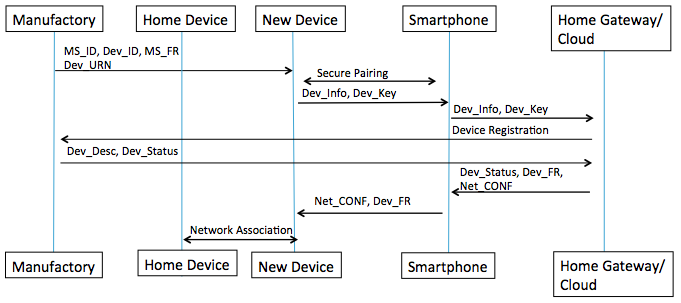
\includegraphics[width=0.8\textwidth]{boot}
  \caption{Secure Bootstrapping Scheme}
  \label{bootscheme}
\end{figure*}

\subsection{Pairing Process}

Pairing process aims to create a secure communication between a new device ($A$) and a smartphone ($B$). It is mainly based on our proposed protocol in~\cite{7158026} which is the best secure and economic solution in its class.  And according to our proof, this protocol could achieve strong security even with a low-bandwidth OOB channel. 

\begin{figure}
  \centering
  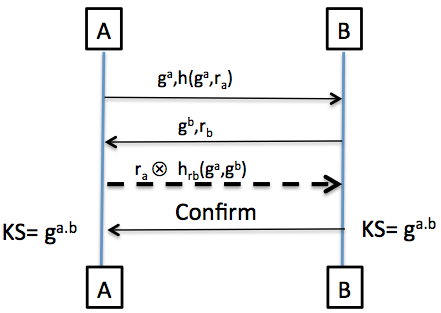
\includegraphics[width=0.35\textwidth]{pairing}
  \caption{Secure Device Pairing Protocol}
  \label{devicepairing}
\end{figure}

The protocol is depicted in the figure ~\ref{devicepairing} and presented as follows. 
\begin{enumerate}
\item $A$ and $B$ generate its own device key $g^a$ and $g^b$ correspondingly. 
\item $A$ picks a random value $r_a$. $B$ picks a random value $r_b$
\item $A$ sends $(g^a,h(g^a,r_a))$ to $B$. $B$ records $g^a$ as Dev\_Key of $A$. 
\item $B$ sends $(g^b,r_b)$ to $A$.
\item $A$ sends $(r_a \otimes h_{r_b}(g^a,g^b) )$ to $B$ over a public out-of-band channel. 
\item $B$ verifies received values and announces the result to $A$. 
\item $A$ confirms by pushing an Accept button. 
\item Both side generate the shared key $KS = g^{a.b}$
\item $A$ sends encrypted information including manufactory identification, device identification, manufactory fingerprinting, and device URN using $KS$ to $B$. 
\end{enumerate}

\subsection{Registration Process}

The registration process happens between a smartphone and a home gateway/a cloud service. In this step, the new device wishes to be validated and to securely receives a device fingerprinting and network settings. The process starts after the smartphone receives a bunch of information from the new device including $MS\_ID$, $Dev\_ID$, $MS\_FR$, and $Dev\_URN$ in previous step. The smartphone enrols the new device to the home gateway. The protocol is illustrated at the figure~\ref{registration}, and presented as below.
\begin{enumerate}
\item The smartphone opens a secure TLS connection to the home gateway using a pre-shared key.
\item The smartphone sends all device information, a device type, and the device's DH key to the home gateway. 
\item The home gateway validates the device information to the manufacture  over a secure HTTPS connection. 
\item The manufactory sends the $Dev\_Desc$ and $Dev\_Status$ to the home gateway.
\item The home gateway possible requests a device registration to the manufactory site if the device has not been registered. 
\item After successful validation and registration, the home gateway generates the $Dev\_FR$, then sends $Dev\_FR$, $Net\_CONF$, $Dev\_Status$, and $SH\_PbKey$ to the smartphone. 
\item The smartphone offers $Net\_CONF$, $Dev\_FR$, and $SH\_Pub$ to the new device.
\item The smartphone cleans all received information when completing the process. 
\end{enumerate}

In case of inaccessible home gateway, the smartphone can forward the registration process to the cloud service as a remote controller. The cloud service then updates new information to the home gateway whenever it is available. 
\begin{figure}
  \centering
  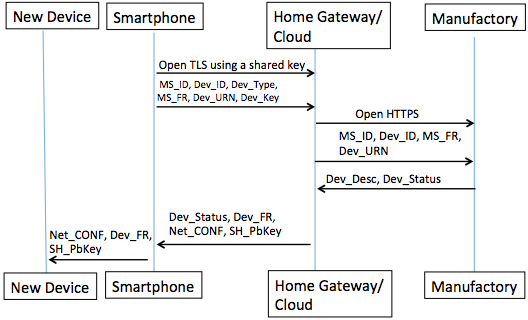
\includegraphics[width=0.5\textwidth]{verification}
  \caption{Registration Process}
  \label{registration}
\end{figure}

\subsection{Association Process}

Network association happens between an authenticated device ($A$) and an authorised device ($B$). The purpose of this process is exchanging the network group key or creating a per-neighbour key between two devices. In this work, we design a network group key exchange protocol.

$A$ wishes to receive the network group key, or $NetPass$, from $B$. The protocol is illustrated in the figure~\ref{netasso}, and happens as follows. In this figure, we denote $Dev_{A}\_FR$ as A's fingerprinting, and $Dev_{B}\_FR$ as B's one. $Dev_{A}\_ID$ and $Dev_{B}\_ID$ denote A's identification and B's identification correspondingly. $g^a$ and $g^b$ are DH keys generated at the pairing process. Apparently, each value is linked to a corresponding device fingerprinting. 

\begin{enumerate}
\item $A$ sends $r_a, Dev_{A}\_FR$ to $B$. 
\item $B$ validates $A$'s fingerprinting using the public key of the home gateway, and produces a shared key $KS = g^{a.b}$.
\item $B$ sends $Dev_{B}\_FR,\{r_a \otimes r_b, NetPass \}_{KS}$ to $A$.
\item $A$ validates $B$'s fingerprinting using the public key of the home gateway, and produces a shared key $KS = g^{a.b}$.
\item $A$ sends $\{r_b\}_{KS}$ to $B$.
\end{enumerate}

\begin{figure}
  \centering
  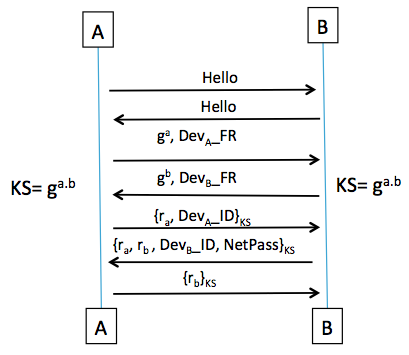
\includegraphics[width=0.4\textwidth]{networkasso}
  \caption{Network Association}
  \label{netasso}
\end{figure}

Note that, it is possible for a home gateway playing in role of an authorised device. 

\subsection{Reassociation Process}
 
The reassociation happens between two authorised devices $A$ and $B$. They wishes to exchange their $NetPass$ securely. When one device receives a $NetPass$ from the other, it checks the $NetPass$'s $ID$. If the new $ID$ is bigger than its current $NetPass$ ID, then the device will update its $NetPass$ key. The protocol is presented below and illustrated at the figure~\ref{renetasso}.

\begin{enumerate}
\item $A$ sends $r_a, Dev_{A}\_FR$ to $B$. 
\item $B$ validates $A$'s fingerprinting using the public key of the home gateway, and produces a shared key $KS = g^{a.b}$.
\item $B$ sends $Dev_{B}\_FR,\{r_a \otimes r_b, NetPass_B \}_{KS}$ to $A$.
\item $A$ validates $B$'s fingerprinting using the public key of the home gateway, and produces a shared key $KS = g^{a.b}$.
\item $A$ sends $\{r_b,NetPass_A\}_{KS}$ to $B$.
\end{enumerate}


\begin{figure}
  \centering
  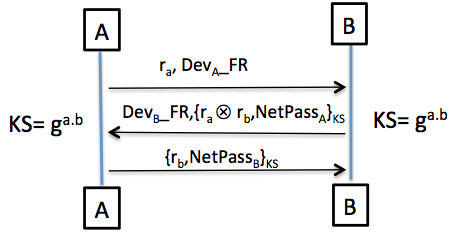
\includegraphics[width=0.4\textwidth]{renetasso}
  \caption{Network Reassociation}
  \label{renetasso}
\end{figure}

By the way of reassociation, whenever a home gateway wishes to update the $NetPass$, it just disconnects and reassociates to neighbour devices to spread the new key. 

\subsection{Reboostrapping}

Rebootstrapping supports re-authentication and rekeying for devices, and allows devices to be administratively switched to a different domain. Therefore, rebootstrapping always requires a smartphone. Whenever rebootstrapping process is demanded by a device, the secure pairing process will be established between the device and the smartphone. After pairing properly, the smartphone chooses a device type then runs the registration process. The home gateway regenerates the device's fingerprinting, then sends $Dev\_Status$, $Dev\_FR$, $Net\_CONF$, and $SH\_PbKey$ to the device via the smartphone. 
 
\section{Security Analysis}\label{validation}

In this section, we present a sketch of proofs of our bootstrapping scheme since this scheme consists of some already-proved protocols. Additionally, these protocols in the bootstrapping scheme are proved in AVISPA~\cite{Armando:2005:ATA:2153230.2153265} as correct protocols. 

Our proposed bootstrapping scheme aims to (i) key agreement between a new device and a smartphone in device pairing process (ii) agreement on device fingerprinting between a new device and a home gateway in the registration process (iii) network group key agreement between an authenticated device and an authorised one in association process. 

\begin{Proposition}\label{ntandsp}
The new device and the smartphone agree on the shared key $K= g^{a.b}$ if the smartphone is not compromised. 
\end{Proposition}

\begin{proof}

According to the assumption on the uncompromised smartphone, this secure pairing protocol is clearly proved in our last work~\cite{7158026}. We also showed that the successful attack probabilities is $Pr[attack] \leq n.\gamma.2^{-k}$ where $n$ is the number of participants on the network, $\gamma$ is the maximum number of sessions for each participant, $k$ is the length of short authenticated string.
\end{proof}

\begin{Proposition}\label{newandsh}
A new device and a home gateway agree on a device fingerprinting $Dev\_FR = \{Dev\_Key, Expires\}_{SH\_PrKey}$. 
\end{Proposition}

\begin{proof}

According to the assumption on uncompromised shared key between the smartphone and the home gateway, attackers cannot open a secure connection to the home gateway/the cloud service with a fake key. Therefore, all messages transmitted on this connection are secured. As a result of this, only regular smartphone can get the device fingerprinting generated by the home gateway/the cloud service. 

Using the result of the proposition~\ref{ntandsp}, whenever a new device gets a device fingerprinting from a regular smartphone, it can ensure this value produced by the home gateway/the cloud service. However, when the device might contacts to attackers, the home gateway does not authenticate this device. Hence,the fake one cannot be validated at the association process. 

\end{proof}

\begin{Proposition}
An authenticated device(A) and an authorised device(B) agree on $NetPass$. 
\end{Proposition}

\begin{proof}

Intuitively, both sides agree on the shared key $KS = g^{a.b}$ by following facts. 
\begin{enumerate}
\item [(i)] The proposition~\ref{newandsh} says the agreement on $Dev_{A}\_FR$ between A and a home gateway.
\item [(ii)] In case of faked smartphones, $A$ might obtain a fake device fingerprinting generated by attackers. However, by the assumption on uncompromised home gateway's private keys, $B$ is able verify $Dev_{A}\_FR$ if it is generated by the home gateway or not. 
\item [(iii)] According to the assumption on uncompromised $B$, $A$ is able to verify $Dev_{B}\_FR$. 
\end{enumerate}

Thus, after two first messages, two principals own the same shared key $KS = g^{a.b}$. Additionally, this protocol is a variant of $Needham$ $Schroeder$ protocol proved in~\cite{674832} using a pre-shared key, $A$ and $B$ can ensure the agreement on $r_a$ and $r_b$. 
Moreover, encrypted by $KS$ in the last message, $NetPass$ cannot be obtained by any attacker. Therefore, $A$ is able to ensure secrecy of $NetPass$. Finally, both sides agree on the secured $NetPass$. 
\end{proof}

\section{Conclusion}\label{conclusion}

Recapping this chapter, not only does our scheme satisfies all of our mentioned requirements, it also provides unique features helpful to bootstrapping devices in some sensitive circumstances. Compared to our scheme, current proposed schemes do not provide the same fashion in term of security, light-weight and adaptability. Particularly, pairing methods such as ~\cite{4159919} and ~\cite{5654588} do not support authorisation and rebootstrapping. In~\cite{Seung2015, Jeanning2013}, QR codes containing an initial key could introduce a weakness point for the system if they are lost. Alternative solutions using pre-shared keys in \cite{JCMjcm0708634642, Cha:2011:LSE:1968613.1968679, Ikram:2009:SLA:1582379.1582583, 6263790, rfc5191} are not sufficiently convenient to users. Finally, lost smartphone in schemes ~\cite{Seung2015, 6934398} leads to leak sensitive information such as pre-shared keys, rebootstrapping information.

Eventually, this chapter offered a novel secure bootstrapping scheme for constrained devices in context of Internet of Things. Precisely, it takes advantage of unsupporting a PKI system, pre-shared keys, and pre-implanted keys. Furthermore, our scheme is not error prone to users since users only participate in the pairing process. In close future, we continue implementing remaining parts of our bootstrapping scheme, and evaluate its usability.





